\documentclass[a4paper,12pt]{article}

%%% Работа с русским языком
\usepackage{cmap}					% поиск в PDF
\usepackage{mathtext} 				% русские буквы в формулах
\usepackage[T2A]{fontenc}			% кодировка
\usepackage[utf8]{inputenc}			% кодировка исходного текста
\usepackage[english,russian]{babel}	% локализация и переносы
\usepackage{indentfirst}
\frenchspacing


%%% Дополнительная работа с математикой
\usepackage{amsmath,amsfonts,amssymb,amsthm,mathtools} % AMS
\usepackage{icomma} % "Умная" запятая: $0,2$ --- число, $0, 2$ --- перечисление

%% Номера формул
%\mathtoolsset{showonlyrefs=true} % Показывать номера только у тех формул, на которые есть \eqref{} в тексте.
%\usepackage{leqno} % Нумерация формул слева

%% Свои команды
\DeclareMathOperator{\sgn}{\mathop{sgn}}

%% Перенос знаков в формулах (по Львовскому)
\newcommand*{\hm}[1]{#1\nobreak\discretionary{}
	{\hbox{$\mathsurround=0pt #1$}}{}}

%%% Работа с картинками
\usepackage{graphicx}  % Для вставки рисунков
\graphicspath{{images/}}  % папки с картинками
\setlength\fboxsep{3pt} % Отступ рамки \fbox{} от рисунка
\setlength\fboxrule{1pt} % Толщина линий рамки \fbox{}
\usepackage{wrapfig} % Обтекание рисунков текстом

%%% Работа с таблицами
\usepackage{array,tabularx,tabulary,booktabs} % Дополнительная работа с таблицами
\usepackage{longtable}  % Длинные таблицы
\usepackage{multirow} % Слияние строк в таблице

%%% Теоремы
\theoremstyle{plain} % Это стиль по умолчанию, его можно не переопределять.
\newtheorem{theorem}{Теорема}[section]
\newtheorem{proposition}[theorem]{Утверждение}

\theoremstyle{definition} % "Определение"
\newtheorem{corollary}{Следствие}[theorem]
\newtheorem{problem}{Задача}[section]

\theoremstyle{remark} % "Примечание"
\newtheorem*{nonum}{Решение}

%%% Программирование
\usepackage{etoolbox} % логические операторы

%%% Страница
\usepackage{extsizes} % Возможность сделать 14-й шрифт
\usepackage{geometry} % Простой способ задавать поля
\geometry{top=15mm}
\geometry{bottom=20mm}
\geometry{left=20mm}
\geometry{right=20mm}
%
%\usepackage{fancyhdr} % Колонтитулы
% 	\pagestyle{fancy}
%\renewcommand{\headrulewidth}{0pt}  % Толщина линейки, отчеркивающей верхний колонтитул
% 	\lfoot{Нижний левый}
% 	\rfoot{Нижний правый}
% 	\rhead{Верхний правый}
% 	\chead{Верхний в центре}
% 	\lhead{Верхний левый}
%	\cfoot{Нижний в центре} % По умолчанию здесь номер страницы

\usepackage{setspace} % Интерлиньяж
%\onehalfspacing % Интерлиньяж 1.5
%\doublespacing % Интерлиньяж 2
%\singlespacing % Интерлиньяж 1

\usepackage{lastpage} % Узнать, сколько всего страниц в документе.

\usepackage{soul} % Модификаторы начертания

\usepackage{hyperref}
\usepackage[usenames,dvipsnames,svgnames,table,rgb]{xcolor}
\hypersetup{				% Гиперссылки
	unicode=true,           % русские буквы в раздела PDF
	pdftitle={Заголовок},   % Заголовок
	pdfauthor={Автор},      % Автор
	pdfsubject={Тема},      % Тема
	pdfcreator={Создатель}, % Создатель
	pdfproducer={Производитель}, % Производитель
	pdfkeywords={keyword1} {key2} {key3}, % Ключевые слова
	colorlinks=true,       	% false: ссылки в рамках; true: цветные ссылки
	linkcolor=violet,          % внутренние ссылки
	citecolor=black,        % на библиографию
	filecolor=orange,      % на файлы
	urlcolor= blue           % на URL
}

\usepackage{csquotes} % Еще инструменты для ссылок

%\usepackage[style=authoryear,maxcitenames=2,backend=biber,sorting=nty]{biblatex}

\usepackage{multicol} % Несколько колонок

\usepackage{tikz} % Работа с графикой
\usepackage{pgfplots}
\usepackage{pgfplotstable}

% Use more than one optional parameter in a new commands
\usepackage{xargs}

% to-do notes
\usepackage[colorinlistoftodos,prependcaption,textsize=tiny]{todonotes}
\newcommandx{\improvement}[2][1=]{\todo[linecolor=Plum,backgroundcolor=Plum!25,bordercolor=Plum,#1]{#2}}

\renewcommand{\phi}{\varphi}
\renewcommand{\epsilon}{\varepsilon}
\usepackage[backend=biber]{biblatex}

\addbibresource{lit.bib}

\makeatletter
\let\@fnsymbol\@arabic
\makeatother

\title{Тензорный метод SSA в задаче декомпозиции многомерных временных рядов}
\author{Сёмкин Кирилл\thanks{semkin.ki@phystech.edu} \and Вадим Стрижов\thanks{vadim.swifton@gmail.com	}}
\date{}


\begin{document}
	
	\maketitle
	
	\begin{abstract}
		
		Декомпозиция временного ряда часто применяется для получения его структуры: разложения на простые и/или интерпретируемые составляющие, выявление периодичности, избавление от шума и т.д. В случае же набора нескольких рядов игнорирование взаимосвязей между ними может приводить к некачественным и ложным разложениям. В данной работе предлагается метод декомпозиции, учитывающий фактор связанности и основанный на классическом методе SSA (Гусеница) и тензорных разложениях. Предложенный подход сравнивается с похожим mSSA, основанным на матричных разложениях, в математических свойствах и при обработке синтетических и реальных данных (потребление электроэнергии, акселерометрия).
		
	\end{abstract}
	
	\section*{Введение}\label{Intro}
	
		Выявление структуры временного ряда --- краеугольная задача математического прогнозирования. Любой метод, независимо от его назначения и цели: предсказание, восстановление пропусков в данных, декомпозиция и т.д., напрямую или косвенно имеет свои предположения насчёт этой структуры. Например, модели стационарных временных рядов (\cite{Box_Jenkins_methodology}, \cite{hamilton1994time}) предполагают рассматриваемый случайный процесс стационарным в широком смысле. Применяемые методы регрессионного анализа (\cite{3b1355aedd1041f1853e609a410576f3}, \cite{Greene2003Econometric}, \cite{enders2010applied})  рассматривают время в качестве независимых переменных (регрессов) и вводят параметрическую модель $ f(\mathbf{\Theta}, t) $, отражающую структуру ряда. Также часто применяются методы на основе динамических систем (\cite{ecfb9dc578be43ae9ee8fc88b8ff9151}, \cite{chen2018neural}, \cite{Tsonis2018}) , предполагающие существование таковой и порождающей наблюдаемый временной ряд напрямую или косвенно. Один из подходов такого типа --- \textbf{SSA}, широко применяется в задачах прогнозирования и разложения на составляющие сигналы.
		
		Классическая постановка задачи декомпозиции временного ряда состоит в его разложении на сезонную, циклическую, тренд и шумовую составляющие. Циклическую и трендовую часть часто объединяют в одну компоненту. Также разложение может быть аддитивным (исходный ряд --- сумма компонент) или мультипликативным (исходный ряд --- произведение компонент). Существует большое количество методов разложения на основе техники скользящего среднего MA (\cite{enders2010applied}, \cite{x11}, \cite{cleveland90}), подбирая сначала авторегрессионную трендовую компоненту, затем усреднением остатка ряда получается сезонная компонента. Данный класс приёмов активно используется в эконометрике и финансах. Также возможно разложение сигнала в ряд фурье по гармоникам или полиномам, и связанные с ним более продвинутые методы (вейвлет преобразование и др.). Данное разложение удобно для амплитудно-частотного анализа сигнала и его фильтрации, но оно имеет недостаток фиксированного базиса функций, по которой раскладывается ряд. Метод SSA же позволяет получить адаптивный базис разложения, связанный с пространством скрытой динамической системы, порождающей наблюдаемый сигнал. Если полученные базисные векторы возможно разделить на группы, отвечающие своему порождаемому сигналу, то мы получаем желанную декомпозицию исходного ряда.
		
		В случае же набора временных рядов, порождённых одной системой и часто одновременно измеренных (например, показания акселерометра и гироскопа; количество реагентов типа А и B при протекании их реакции и т.д.), их разложение порознь обычными методами скорей всего ни отразит их общей структуры, ни даст качественных, интерпретирующихся компонент. Для решения данной проблемы существует простая модификация 'Гусеницы' - \textbf{mSSA}, описание которой будет приведено ниже. Она успешно применяется на практике: например, изучение фазовой синхронизации \cite{PhysRevE.84.036206} или восстановление пропусков в временных рядов \cite{agarwal2020multivariate}.
		
	    В данной работе вводится ещё одна модификация: \textbf{tSSA}, в которой предлагается использовать мощь тензорных разложений вместо матричных. В большинстве своём для них нет простых и понятных алгоритмов, но существуют достаточно быстрые приближённые, что в случае больших выборок будет вычислительно эквивалентно матричным. С другой стороны, представление временных рядов в виде тензора и его декомпозиция потенциально более выразительна и способна  выявить более тонкие взаимодействия между рядами. Применение и исследование данного метода можно найти в \cite{6661921}, \cite{6834801}, где авторы сворачивают одномерный сигнал ЭКГ мозговой активности в трёхмерный тензор и получают его разложение по IMFs (intrinsic mode functions) определённых частот. В работе \cite{app7040418} авторы применяют ту же технику но для анализа сигнала отклика механических систем, а также предлагают сведение задачи тензорного разложения к задаче выпуклой оптимизации. В работах \cite{10122507} и \cite{FU2023115} исследователи работают с \href{https://en.wikipedia.org/wiki/Hyperspectral_imaging}{гиперспектральными изображениями}, которые сами по своей природе представляются в виде многомерных массивов, и тензорное разложение позволяет учесть не только взаимодействие в цветовых каналах изображения, но и пространственно-спектральное. Метод успешно применяется для сегментации изображений земной поверхности. 
	    
	    Далее будет дано математическое описание алгоритмов mSSA и tSSA, их особенности и сравнение в подходах к декомпозиции многомерных рядов. После данные методы тестируются на разложении набора синтетических рядов (гармонические функции с разными частотами), а также на реальных данных: потребление электроэнергии частным домохозяйством в течении года и данными акселерометра движущегося пешехода. Анализируется ошибка, возникающая при разложении рядов, интерпретируемость разложения, качество предсказания на отложенных значениях выборки. 
	    
	    \section*{Теоретическая часть}
	    
	    	Пусть имеем набор временных рядов $ \{x_i(t_j)\}_{i = 1}^{m} $, где сетка по времени $ t_j \in \overrightarrow{1, N} $. Стоит задача разложения временных рядов на аддитивные компоненты: 
	    	
	    	\begin{gather*}
	    		x_1(t) = f_1(t) + f_2(t) + \ldots + f_{n_1}(t) \\
	    		x_2(t) = g_1(t) + g_2(t) + \ldots + g_{n_2}(t) \\
	    			   ...
	    	\end{gather*}
	    	
	    	Формулировка задачи слишком общая, ведь таких разложений для произвольной функции можно построить сколь угодно много и каким угодно способом: можно раскладывать по индикаторным функциям (любую измеримую функцию можно так разложить), можно в ряды Фурье, и т.д. Мы же будем полагаться на свойства вводимых далее методов с некоторыми предположениями для поиска разложения.
	    
	    	\subsection*{Метод SSA}
	    	
	    	Пусть имеем пока один времнной ряд. Подход 'Гусеницы' предполагает наличие некоторой динамической системы, порождающей наблюдаемый ряд, и опирается на теорему Такенса об аппроксимации многообразия, в котором лежат траектории системы, \textit{векторами временных задержек} (\cite{citeulike:2735031}). Для построения этих векторов выбирается длина окна $ L $, далее это окно 'прикладывается' к разным частям временного ряда (см. рис.\ref{pic:hankel_build} ). Формально k-ый вектор задержек есть $ \mathbf{x}_k = ( x(t_k) \  x(t_{k+1}) \  \ldots \  x(t_{k + L - 1}) ) $. Далее данные вектора собираются в матрицу $ T_{ij} $ по столбцам, у которой в результате все антидиагональные элементы $ i + j = const $ равны. Такие матрицы называются \textit{ганкелевой}, а в терминах временных рядов матрица $ T $ называется \textit{траекторной} или матрицей задержек.
	    	
	    	\begin{figure}
	    		\centering
	    		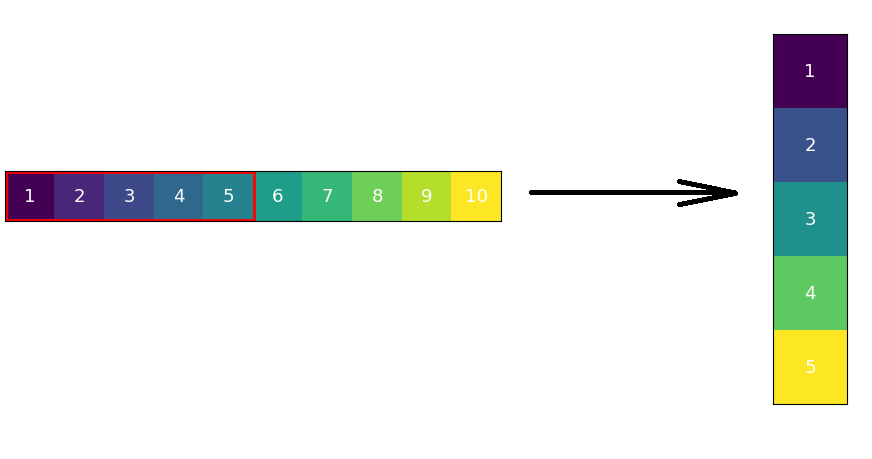
\includegraphics[width=0.6\textwidth, keepaspectratio]{../figs/first_round}
	    		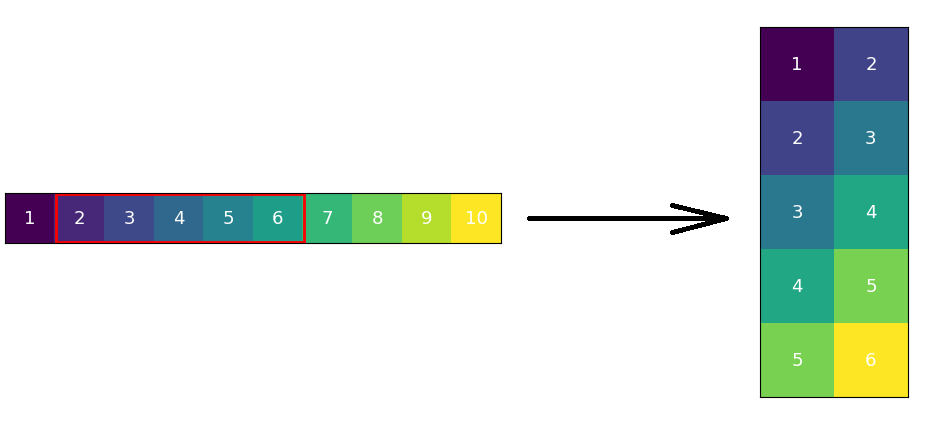
\includegraphics[width=0.6\textwidth, keepaspectratio]{../figs/second_round.png}
	    		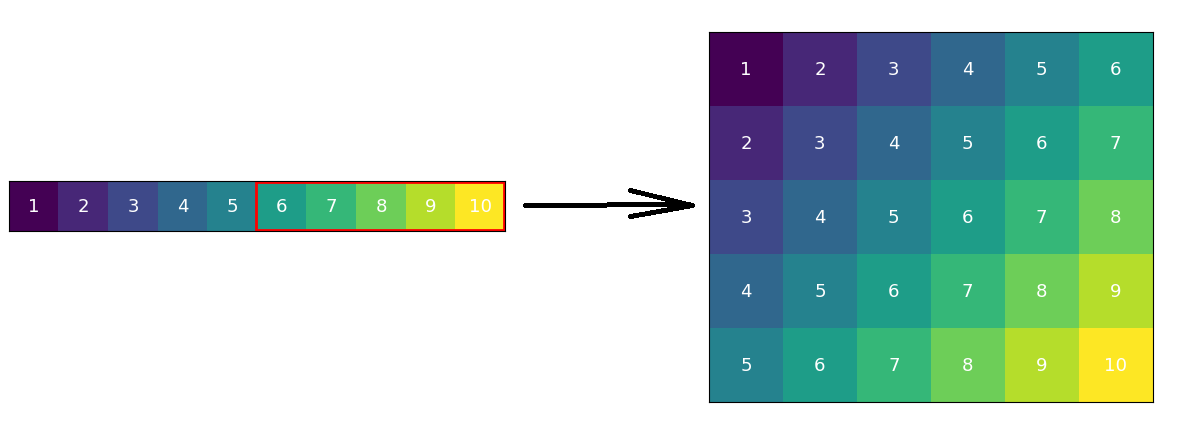
\includegraphics[width=0.6\textwidth, keepaspectratio]{../figs/last_round.png}
	    		\caption{Построение ганкелевой матрицы}\label{pic:hankel_build}
	    	\end{figure}
	    	
	    	Далее к матрице применяется SVD-разложение $ T = \sum\limits^{r} \sigma_i \mathbf{u}_i \mathbf{v}_i $ (знак транспонирования для $ \mathbf{v}_i $ опускается), получая таким образом тот самый адаптивный ортонормированный базис $ \{\mathbf{u}_i\}_{i=1}^r $ в пространстве векторов задержек. Компоненты с малыми $ \sigma_i $ интерпретируются как шумовые.
	    	
	    	Для декомпозиции исходного ряда предлагается следующее: пусть $ x(t) = f_1(t) + f_2(t) $ и пусть мы построили ганкелевы матрицы $ X_1, X_2 $ для $ f_1(t) $ и $ f_2(t) $, тогда $ T = X_1 + X_2 $. Как известно, SVD-разложение матриц единственно (разложение по ортонормированному базису), т.е. для матриц $ X_1 $ и $ X_2 $ это разложение по тем же базисам $ \{\mathbf{u}_i\}_{i=1}^r, \  \{\mathbf{v}_i\}_{i=1}^r $. Главное предположение здесь --- возможность разделить эти базисы на две \underline{непересекающиеся} группы:  $ ( \{\mathbf{u}^1_i\}_{i=1}^{r_1}, \, \{\mathbf{v}^1_i\}_{i=1}^{r_1} ) $ и $ ( \{\mathbf{u}^2_i\}_{i=1}^{r_2}, \, \{\mathbf{v}^2_i\}_{i=1}^{r_2} ) $, где $ r_1 + r_2 = r $. Тогда возможно вычленить декомпозицию исходного ряда из его сингулярного разложения:
	    	
	    	\begin{equation*}
	    		 T = \sum\limits_i^{r} \sigma_i \mathbf{u}_i \mathbf{v}_i = \sum\limits_i^{r_1} \sigma_i^1 \mathbf{u}_i^1 \mathbf{v}_i^1 + \sum\limits_i^{r_2} \sigma_i^2 \mathbf{u}_i^2 \mathbf{v}_i^2 = X_1 + X_2
	    	\end{equation*}
	    	
	    	Получив $ X_1, X_2 $ можно однозначно восстановить $ \{f_1(t_j)\}, \{f_2(t_j)\} $, для этого достаточно взять первый столбец и последнюю строки в этих матрицах и соединить в один вектор друг за другом --- это мгновенно следует из способа построения матриц векторов задержек и их ганкелевой структуры. Таким же образом можно разделять спектральное разложение на большее число групп и по той же процедуре извлекать составляющие сигнала, если гипотеза возможности такого разделения верна.
	    	
	    	Вводимое предположение имеет следующий смысл: т.к. вектора задержек для $ f_1(t) $ и $ f_2(t) $ лежат в ортогональных друг другу пространствах, порождённых $ \{\mathbf{u}^1_i\}_{i=1}^{r_1} $ и $ \{\mathbf{u}^2_i\}_{i=1}^{r_2} $, то и исходные вектора задержек двух рядов ортогональны друг другу:
	    	
	    	\[
	    		 f_1(t_i) f_2(t_i) + \ldots + f_1(t_{i + L - 1}) f_2(t_{i + L - 1}) = <f_{1, L}, f_{2, L}> = 0, \  \forall i \in \overrightarrow{1, N - L + 1}
	    	\]
	    	
	    	 С точки зрения динамических систем, между векторами задержек и многообразием траекторий скрытой системы существует диффеоморфизм, таким образом существование предполагаемого разделение говорит о разложимости скрытого многообразия в прямую сумму подпространств.
	    	
	    	Как показано в подробной книге о методе SSA \cite{ecfb9dc578be43ae9ee8fc88b8ff9151}, многие простые типы функций невозможно строго разделить таким образом. Тем не менее, в асимптотическом приближении $ N \to \infty, L \to \infty $ они разделяются, т.е. их корреляция в этом случае $ <f_{1, L}, f_{2, L}> \to 0 $, см. табл.\ref{tab:asympt_devis}. Также там показано, что если $ \exists \tilde{L}: \forall L > \tilde{L} \hookrightarrow rank(T) = r = const $, то исходный ряд в точности описывается авторегрессионной моделью.
	    	
	    	\begin{table}[h]
	    		\centering
	    		\caption{Асимптотическая разделимость компонент (Golyandina)}\label{tab:asympt_devis}
	    		\begin{tabular}{|c|c|c|c|c|c|}
	    			\hline
	    			& const & cos & exp & exp (cos) & ak + b \\ \hline
	    			const     & -     & +   & +   & +         & -      \\ \hline
	    			cos       & +     & +   & +   & +         & +      \\ \hline
	    			exp       & +     & +   & +   & +         & +      \\ \hline
	    			exp (cos) & +     & +   & +   & +         & +      \\ \hline
	    			ak + b    & -     & +   & +   & +         & -      \\ \hline
	    		\end{tabular}
	    	\end{table}
	    	
	    	Т.к. любые данные содержат в себе ошибки (погрешности измерений, неточности вычислений и т.д.), даже идеально разделяемые ряды на практике не получится чётко разделить по спектральному разложению. Поэтому применяется простая процедура: полученные в ходе разделения главных компонент $ X_1, X_2 $ \textit{ганкелизуются}, т.е. каждая антидиагональ матриц усредняется и заменяется на это среднее.\improvement{втавить оценку ошибки такого приближения}
	    	
	    	%TODO: втавить оценку ошибки такого приближения
	    	
	    	Таким образом оценивать полученную декомпозицию можно по получившейся невязке. Также часто для разделения главных компонент используют \textit{относительную близость спектральных чисел}, т.е. по сути происходит их кластеризация. В той же \cite{ecfb9dc578be43ae9ee8fc88b8ff9151} есть некоторые обоснования этого для некоторых классов функций.
	    	
	    	
			\subsection*{Метод mSSA}
			
			Пусть теперь имеем $ m $ временных рядов $ \{x_i(t_j)\}_{i = 1}^{m} $, где $ t_j \in \overrightarrow{1, N} $. Предполагая ту же гипотезу о природе порождения этих сигналов, будет действовать похожим на SSA способом. Для этого опять выбираем длину окна $ L $ и строим траекторные матрицы для каждого ряда $ T_1, T_2, \ldots , T_m  $. Теперь конкатенируем все матрицы в одну $ T = [T_1 \  T_2 \ldots T_m] $, которую далее раскладываем с помощью SVD:
			
			\begin{equation*}
				T = \sum\limits_i^{r} \sigma_i \mathbf{u}_i \mathbf{v}_i \Leftrightarrow \begin{cases}
					T_1 = \sum\limits_i^{r} \sigma_i \mathbf{u}_i \mathbf{v}_i^1 \\
					T_2 = \sum\limits_i^{r} \sigma_i \mathbf{u}_i \mathbf{v}_i^2 \\
					\ldots \\
					T_m = \sum\limits_i^{r} \sigma_i \mathbf{u}_i \mathbf{v}_i^m
				\end{cases}
			\end{equation*}
			
			Здесь каждая главная компонента в пространстве строк $ \mathbf{v}_i $ представляется в виде конкатенации: $ \mathbf{v}_i = (\mathbf{v}_i^1 \ldots \mathbf{v}_i^m) $. Т.о. получаем некоторое разложение траекторных матриц, которое не является SVD-разложением в общем случае (т.к. компоненты $ \mathbf{v}_i^k $ не обязаны быть ортогональны между собой). Тем не менее базис столбцов у всех сигналов одинаковый $ \{\mathbf{u}_i\}_{i=1}^r $ и ортонормированный, 'сингулярные' числа тоже одинаковые. Таким образом общее столбцовое пространство связывает траекторные матрицы каждого ряда и учитывает их общую природу порождения.
			
			Дальнейший ход действий для декомпозиции аналогичен методу SSA. Можно рассматривать разложение каждой траекторной матрицы отдельно, но т.к. все они имеют общий набор 'сингулярных' чисел, и группировка главных компонент часто делается на их основе, то разделение на группы происходит одинаковое для всех траекторных матриц. Получаем итоговое разложение каждого сигнала в виде:
			
			\begin{gather*}
				x_1(t) = \hat{f}_1(t) + \hat{f}_2(t) + \ldots + \hat{f}_{n}(t) \\
				x_2(t) = \hat{g}_1(t) + \hat{g}_2(t) + \ldots + \hat{g}_{n}(t) \\
				... \\
				x_m(t) = \hat{h}_1(t) + \hat{h}_2(t) + \ldots + \hat{h}_{n}(t)
			\end{gather*}
			
			\subsection*{Метод tSSA}
			
			Данный подход основан на сборке того же набора рядов $ \{x_i(t_j)\}_{i = 1}^{m} $ в тензор и применения уже \textit{тензорного} разложения вместо рассматриваемого до этого SVD. Сразу отметим, что способов упаковки и разложений для тензоров можно предложить огромное количество (для базового ознакомления можно, например, обратиться к \cite{rabanser2017introduction}; также см. предлагаемые работы в \nameref{Intro}), являясь ещё скудно изученной областью в приложении к временным рядам.
			
			 В данной работе предлагается вдохновлённый классическим SSA способ получения \textit{траекторного тензора} $ \mathbf{T} $: как и в mSSA, строятся траекторные матрицы для каждого ряда $ T_1, \ldots, T_m $, после чего данные матрицы состыковываются друг с другом по третьему измерению (индексу) тензора. Т.о. измерениям $ \mathbf{T} $ соответствуют столбцы и строки временных задержек, а также номер сигнала. Далее, к полученному тензору применяется \textit{каноническое разложение} (Canonical polyadic decomposition, CPD), как наиболее схожее с SVD разложение (см. рис.\ref{pic:cpu_dec}).
			 
			 \begin{figure}[h]
			 	\centering
			 	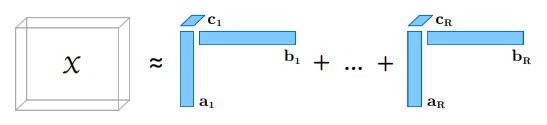
\includegraphics[width=0.6\textwidth, keepaspectratio]{../figs/cpu_decomp}
			 	\caption{Иллюстрация канонического разложения}\label{pic:cpu_dec}
			 \end{figure}
			 
			 С математической точки зрения это выглядит так:
			 
			 \begin{equation*}
			 	\mathbf{T} = \sum\limits_i^{r} \mathbf{a}_i \otimes \mathbf{b}_i \otimes \mathbf{c}_i \Leftrightarrow \begin{cases}
			 		T_1 = \sum\limits_i^{r} \mathbf{c}_i[1] \cdot \mathbf{a}_i  \mathbf{b}_i  \\
			 		T_2 = \sum\limits_i^{r} \mathbf{c}_i[2] \cdot \mathbf{a}_i  \mathbf{b}_i \\
			 		\ldots \\
			 		T_m = \sum\limits_i^{r} \mathbf{c}_i[m] \cdot \mathbf{a}_i  \mathbf{b}_i 
			 	\end{cases}
			 \end{equation*}
			 
			 Здесь записано разложение исходного тензора в сумму тензорных произведений набора векторов $ \mathbf{a}_i, \mathbf{b}_i, \mathbf{c}_i $, которые можно для удобства состыковать в матрицы $ A, B, C $. Если зафиксировать третий индекс, то получим разложение каждой траекторной матрицы $ T_i $, где $ \mathbf{c}_i[k] $ --- это $ k $-ая компонента вектора $ \mathbf{c}_i $. Таким образом разложение происходит по одному базису как для столбцов, так и для строк у каждой матрицы задержек! Роль же сингулярных чисел играют строки матрицы $ C $. Дальнейший ход действий для получения декомпозиции аналогичен SSA.
			 
			 Полученное разложение обладает \textit{рядом преимуществ} по сравнению с mSSA: теперь имеем общий базис как у столбцов, так и у строк матриц $ T_i $, что ещё сильнее связывает каждый сигнал; тем более строки у $ T_i $ - это те же вектора задержек, только другой размерности, поэтому странно раскладывать их для каждой $ T_i $ по своему базису, если столбцы раскладываются по одному. Также данное разложение более гибкое, т.к. для каждой матрицы задержки имеется свой набор $ \mathbf{c}_i[k], \,  k \in \overrightarrow{1, r} $ 'сингулярных' чисел, что позволяет каждому сигналу подстроиться под базисные векторы индивидуально. Таким образом каждую траекторную матрицу можно раскладывать также индивидуально, что было затруднительно в mSSA. Ещё одним положительным моментом является свойство CPD-разложения: при затратно проверяемых, но весьма необременительных условиях оно единственно.
			 
			 
			 Тем не менее есть и некоторые недостатки по сравнению с матричным разложением: теперь базисы в пространстве столбцов не составляют ортогональную систему (чего не скажешь о mSSA), в пространстве строк аналогично (у mSSA та же проблема). Поэтому имеет смысл объединять слишком скоррелированые векторы в этих базисах. Также их необходимо нормировать для преемственности с предыдущими методами, нормы векторов скорректируют изначальные 'сингулярные' числа (далее по умолчанию предполагаем нормированность). Ещё эти числа могут быть отрицательными, что уменьшает их интерпретируемость.
			 
			 О других проблемах рассмотренных методов ещё немного в следующем разделе.
			 
			 
			 \subsection*{Трудности рассмотренных методов}
			 
			 	В данном разделе хочется априори проанализировать на несколько 'белых пятен' и проблем предложенных алгоритмов.
			 	
			 	\subsubsection*{Проблема выбора группировки}
			 	
			 		Как и в обычном SSA, как и в других рассматриваемых методах, необходимо группировать полученную сумму факторов в разложении матриц $ T_i $. Для SSA и mSSA это возможно делать по близости сингулярных чисел, хотя нет абсолютно никакой гарантии в правильности данного подхода. В tSSA из-за того, что эти числа могут быть отрицательными и более разреженными, такой метод отбора затруднителен. Качество полученной группировки можно оценить по совокупной ошибке при ганкелизации полученных факторов. Но предложить быстрый метода хорошего выбора пока затруднительно. Возможно в tSSA разложении можно разбивать полученные базисные векторы на почти ортогональные подсистемы, что будет служить знаком существования возможности группирования. В других методах столбцовый базис уже составляет ортогональную систему.
			 		
			 	\subsubsection*{Сложность вычислений}
			 	
			 		Предложенные методы работают с разложением матриц и тензоров, что при больших объёмах выборок и выбора длины окна $ L $ может привести к невозможности их использования, по крайней мере стандартных алгоритмов. Например, в табл.\ref{tab:svd_time}  приведено время работы и требования по памяти для SVD-разложения из библиотеки \textit{scipy}. Поэтому для размеров временных рядов $ \gtrsim 10^4 $ необходимо искать более продвинутые решения.
			 		
			 		\begin{figure}[h]
			 			\centering
			 			\caption{Сложность SVD-разложения (scipy)}\label{tab:svd_time}
			 			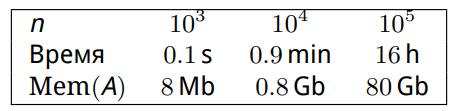
\includegraphics[width=0.6\textwidth, keepaspectratio]{../figs/svd_time.png}
			 		\end{figure}
			 		
			 		Для CPD-разложения всё сложней. Несмотря на его хорошие свойства, вычисление канонического ранга $ r $ является NP-трудной задачей. Поэтому при  применении tSSA его необходимо подбирать. Из-за неточности этого подбора возможна большая ошибка аппроксимации полученным разложением исходного тензора $ \mathbf{T} $, а слишком больший выбор $ r $ приводит к большому времени вычисления и потребляемой памяти. Достаточно быстрый итерационный приближённый алгоритм ALS (Alternating Least Squares) всё равно оперирует матрицами, их свёртками и нахождениями минимума матричных функций, что катастрофично для тензоров больших размеров.
			 
			 \subsection*{Вычислительный эксперимент}
			 
			 
			 \subsection*{Анализ ошибки}
			
			
		
		\newpage
		\printbibliography
	
\end{document}